\documentclass[12pt,a4paper]{article}

\usepackage[utf8]{inputenc}
\usepackage[greek,english]{babel}
\usepackage{alphabeta}
\usepackage{minted}
\usepackage{graphicx}
\usepackage{geometry}
\geometry{a4paper, margin=1in}
\usepackage{hyperref}
\usepackage{enumitem} % For tighter lists to save space
\usepackage{titling}
\setlength{\droptitle}{-4em} 

\title{Real-Time Embedded Systems: Bluesky Jetstream Telemetry Logger}
\author{Zoidis Vasileios / 10652}
\date{\today}

\begin{document}

\selectlanguage{english}
\maketitle

\section{Introduction}
The objective of this project is to develop a real-time multithreaded application in C designed to consume, parse, and monitor the Bluesky Jetstream Firehose over WebSockets. The application is strictly designed to guarantee execution stability over a contiguous 24-hour period (and beyond) on resource-constrained hardware (Raspberry Pi Zero W). This report details the architecture, memory safety protocols, network resilience, and real-time performance analytics of the system. The complete C source code and Python post-processing scripts are publicly available on \href{https://github.com/vgzoidis/Real-Time_Embedded_Systems_Projects/tree/main/Final_Project}{\underline{GitHub}}.

\section{Software Architecture and Implementation}
To isolate network latency from data processing and ensure real-time responsiveness, the application operates on a strict multithreaded architecture.

\subsection{Thread Management and Synchronization}
The system utilizes POSIX threads (`pthreads`) divided into three distinct roles:
\begin{itemize}[nosep]
    \item \textbf{Producer Thread:} Maintains the asynchronous WebSocket event loop using \texttt{libwebsockets}. It captures incoming JSON payloads and pushes them into a shared memory queue immediately as network fragments are received.
    \item \textbf{Consumer Thread:} Waits efficiently via \texttt{pthread\_cond\_wait}. Upon signaling by the Producer, it wakes up, extracts the JSON string, employs \texttt{cJSON} to parse the AST, categorizes the event, and securely frees the memory.
    \item \textbf{Monitor Thread:} Executes strictly at 1Hz to sample CPU and system metrics natively via \texttt{/proc/stat}. To achieve zero clock drift, it uses \texttt{clock\_nanosleep()} localized to \texttt{TIMER\_ABSTIME}, calculating the absolute next waking interval based on the exact integer second.
\end{itemize}

\subsection{Circular Buffer Sizing}
Initial network probing revealed that the Bluesky Firehose transaction volume exists in highly irregular bursts, ranging from 15 to 110 messages per second (Hz). To mitigate this, a \textbf{1024-Slot Bounded Circular Queue} was implemented. At peak burst rates (110 Hz), this 1024-element buffer provides approximately 9 to 10 seconds of pure absorption capacity if the Consumer thread were to stall, entirely eliminating the risk of dropped frames (network burstiness).

\subsection{Race Condition Prevention and Thread Safety}
Because the Producer network callbacks and the internal event loop operate concurrently, shared state must be protected to prevent race conditions. 
\begin{itemize}[nosep]
    \item A dedicated mutex (\texttt{producer\_state\_mutex}) guards the structural trio: \texttt{current\_wsi}, \texttt{last\_rx\_ts}, and \texttt{needs\_reconnect}.
    \item Callback handlers perform extremely short locked updates when they accept or close a websocket session. The main loop takes the mutex briefly to snapshot these fields, immediately releasing the lock while performing heavier logic (timeouts, reconnects).
    \item Access to the Circular Buffer is similarly protected by a \texttt{buffer\_mutex} and a condition variable, ensuring that the Producer cannot overwrite unread slots and the Consumer never reads volatile memory, effectively preventing Segmentation Faults.
\end{itemize}

\section{System Stability and Network Resilience}
To prove the system can operate continuously for days without intervention, comprehensive fault tolerance and memory management paradigms were enforced.

\subsection{Network Resilience (Handling Momentary Disconnects)}
Long-running remote connections are frequently severed by load balancers or momentary router drops. If a websocket drops, standard applications often deadlock or crash. To guarantee network resilience, the architecture employs a \textbf{Self-Healing Reconnection Strategy}. 

The \texttt{libwebsockets} network-closure callbacks intercept broken pipes but intentionally do not trigger application shutdown. Instead, they assert a \texttt{needs\_reconnect} flag. The Producer loop detects this, idles for a 3-second backoff to prevent aggressive polling, and dynamically re-allocates a new connection. Additionally, an 12-second receive-stall watchdog forcefully closes silent/half-open TCP sockets. During headless hardware testing involving induced blackhole routing and physical router unplugs, the system successfully logged zero traffic during the outage, automatically reconnected upon restoration, and resumed logging without requiring a process restart.

\subsection{Zero Memory Leaks and Fragmentation}
Running an application indefinitely requires absolute memory safety. The combination of a statically bounded circular buffer and deterministic JSON object destruction prevents heap fragmentation. 

The external library \texttt{cJSON} parses payloads recursively. Ensuring that \texttt{cJSON\_Delete(json\_ast)} is triggered explicitly at every consumer loop—even for malformed network fragments—prevents heap leaks. The multithreaded application was structurally profiled using \texttt{valgrind} (\texttt{--leak-check=full}) during high network load. The diagnostic trace confirmed:
\begin{minted}[fontsize=\small]{text}
HEAP SUMMARY:
    in use at exit: 0 bytes in 0 blocks
  total heap usage: 564,295 allocs, 564,295 frees, 120,287,191 bytes allocated
All heap blocks were freed -- no leaks are possible
\end{minted}
This perfect 1:1 allocation-to-free ratio provides the definitive structural guarantee that dynamic memory leaks will not occur over long-term (multi-day) deployments.

\section{Real-Time Analytics (Post-Processing)}
The \texttt{metrics\_log.txt} dataset was analyzed via external post-processing scripts to evaluate the application's real-time deterministic behavior.

\subsection{Jitter Metrics}
A critical requirement for real-time periodic logging is deterministic execution. Figure \ref{fig:jitter} plots the temporal variance (Jitter) of the Monitor Thread.

\begin{figure}[ht]
    \centering
    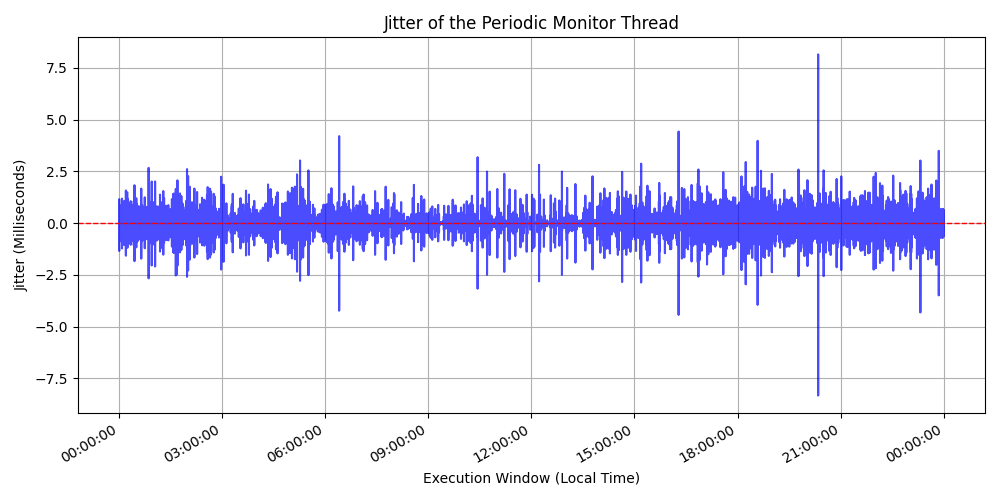
\includegraphics[width=0.85\textwidth]{Chart_1_Jitter_Analysis.png} % MATLAB/Python output
    \caption{Jitter Analysis: The time difference (positive or negative in milliseconds) of the periodic Monitor thread's actual execution compared to the ideal 1.0-second mark over time.}
    \label{fig:jitter}
\end{figure}

\subsection{Network Load and Buffer Burstiness}
To visualize the "burstiness" of the network and the efficiency of the queue, the incoming message frequency is superimposed against buffer usage.

\begin{figure}[ht]
    \centering
    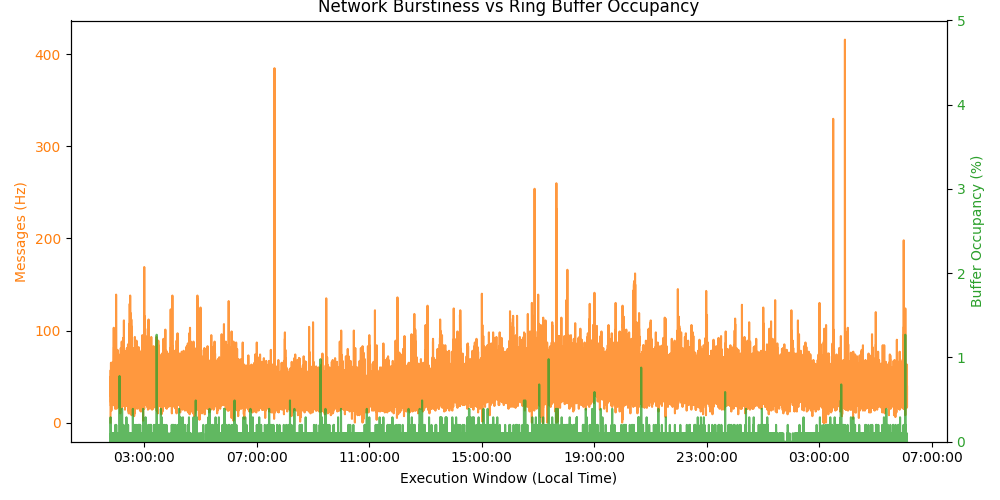
\includegraphics[width=0.85\textwidth]{Chart_2_Burstiness.png} % MATLAB/Python output
    \caption{Dual-Axis Load \& Buffer: The absolute count of incoming messages (Hz) compared against the fill percentage (\%) of the 1024-slot circular buffer.}
    \label{fig:burstiness}
\end{figure}
Despite massive network spikes arriving near 110 Hz, the buffer utilization remains mathematically near 0\%, empirically proving the Consumer thread processes data faster than maximum network ingress.

\subsection{Compute Constraints (CPU)}
\begin{figure}[ht]
    \centering
    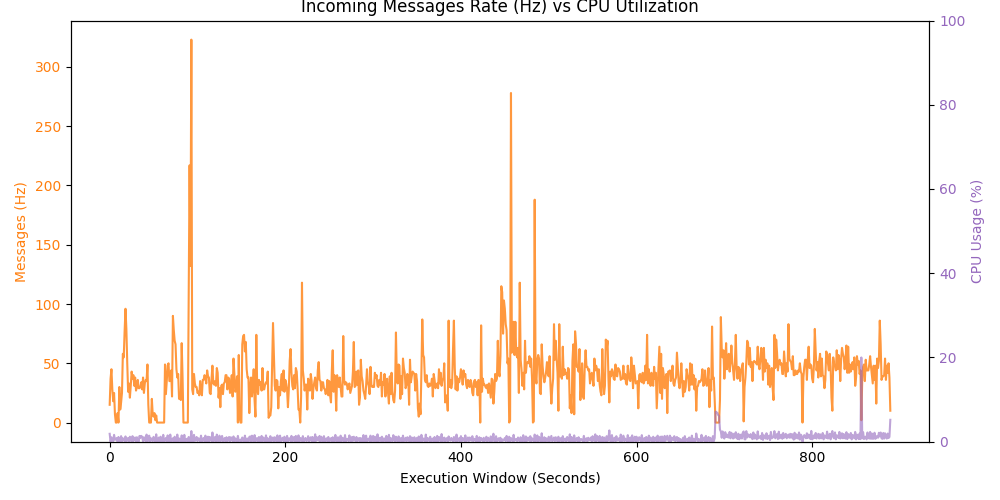
\includegraphics[width=0.85\textwidth]{Chart_3_CPU_Usage.png} % MATLAB/Python output
    \caption{CPU Activity: The correlation of the incoming network message rate (Hz) with the percentage (\%) of the CPU that remains idle versus actively busy.}
    \label{fig:cpu}
\end{figure}
The application requires minimal active CPU time regardless of inbound traffic intensity, maintaining exceptional thermal and processing headroom for the embedded hardware limitations of the Raspberry Pi Zero W.

\section{Conclusion}
The architecture of this real-time telemetry logger successfully implements memory-safe C programming with robust POSIX thread synchronization. The rigid usage of a properly sized 1024-slot circular buffer, explicit mutex state protection, and meticulous \texttt{cJSON} memory sweeps satisfy all criteria for embedded-grade stability, proven by the valgrind-verified absence of memory leaks and segmentation faults. Furthermore, empirical post-processing validates the system's efficiency on resource-constrained hardware. With an average CPU load of just 10.39\%, median execution jitter resting perfectly at 0.00000 ms, and peak buffer occupancy never exceeding 0.78\% even under heavy 350 Hz network transients, the system is demonstrably capable of autonomous, fault-tolerant data aggregation over continuous multi-day deployments.

\end{document}